\chapter{Design and coding}
\label{cap:design-coding}

\intro{In this chapter we will describe the design and coding of the project.
We will start by describing the technologies and tools used, then we will
describe the software life cycle, the design and the design patterns used and
finally we will describe the coding phase.}


\section{Technology and tools}
\label{sec:technology-tools}

In the following sections we will describe the technologies and tools used in
the project.
\subsection*{Python}
\label{subsec:python}
Python is a programming language that lets you work quickly and integrate
systems more effectively. It is a high-level programming language, with
applications in numerous areas, including web programming, scripting, scientific
computing, and artificial intelligence. It is very popular and used by many
companies, such as Google, Facebook, Instagram, Spotify, Netflix, Dropbox, and
many others. It is also used in the development of many open source projects,
such as Blender, GIMP, Inkscape, and many others. It is a very versatile
language, with a very large community and a very large number of libraries
available. It is also a very simple language to learn, with a very simple
syntax, which makes it very readable and easy to understand. It is also a
language that is constantly evolving, with new versions released every year,
which makes it always up to date and with the latest technologies.

\subsection*{CUDA}
\label{subsec:cuda}
CUDA is a parallel computing platform and programming model developed by NVIDIA
for general computing on graphical processing units (GPUs). With CUDA, developers
are able to dramatically speed up computing applications by harnessing the power
of GPUs. In GPU-accelerated applications, the sequential part of the workload
runs on the CPU – which is optimized for single-threaded performance – while the
compute intensive portion of the application runs on thousands of GPU cores in
parallel. When using CUDA, developers program in popular languages such as C,
C++, Fortran, Python and MATLAB and express parallelism through extensions in
the form of a few basic keywords.

\subsection*{CuDNN}
\label{subsec:cudnn}
The NVIDIA CUDA® Deep Neural Network library (cuDNN) is a GPU-accelerated library
of primitives for deep neural networks. cuDNN provides highly tuned
implementations for standard routines such as forward and backward convolution,
pooling, normalization, and activation layers. cuDNN is part of the NVIDIA Deep
Learning SDK.

\subsection*{ML libraries}
\label{subsec:mllib}
\subsubsection*{TensorFlow}
\label{subsubsec:tensorflow}
TensorFlow is an end-to-end open source platform for machine learning. It has a
comprehensive, flexible ecosystem of tools, libraries and community resources
that lets researchers push the state-of-the-art in ML and developers easily
build and deploy ML powered applications.
\subsubsection*{PyTorch}
\label{subsubsec:pytorch}
PyTorch is an open source machine learning library based on the Torch library,
used for applications such as computer vision and natural language processing,
primarily developed by Facebook's AI Research lab (FAIR). It is free and open
source software released under the Modified BSD license. Although the Python
interface is more polished and the primary focus of development, PyTorch also
has a C++ interface.
\subsubsection*{Keras}
\label{subsubsec:keras}
Keras is a high-level neural networks \gls{apig}, written in Python and capable of
running on top of TensorFlow, CNTK, or Theano. It was developed with a focus on
enabling fast experimentation. Being able to go from idea to result with the
least possible delay is key to doing good research.
\subsubsection*{OpenCV}
\label{subsubsec:opencv}
OpenCV (Open Source Computer Vision Library) is an open source computer vision
and machine learning software library. OpenCV was built to provide a common
infrastructure for computer vision applications and to accelerate the use of
machine perception in the commercial products. Being a BSD-licensed product,    
OpenCV makes it easy for businesses to utilize and modify the code. The library
has more than 2500 optimized algorithms, which includes a comprehensive set of
both classic and state-of-the-art computer vision and machine learning
algorithms. These algorithms can be used to detect and recognize faces, identify
objects, classify human actions in videos, track camera movements, track moving
objects, extract 3D models of objects, produce 3D point clouds from stereo
cameras, stitch images together to produce a high resolution image of an entire
scene, find similar images from an image database, remove red eyes from images
taken using flash, follow eye movements, recognize scenery and establish markers
to overlay it with augmented reality, etc. OpenCV has more than 47 thousand
people of user community and estimated number of downloads exceeding 18 million.
The library is used extensively in companies, research groups and by governmental
bodies.
\subsection*{GANs Models}
\label{subsec:gans-models}
\subsubsection*{Pix2Pix}\footcite{paper:pix2pix}
\label{subsubsec:pix2pix}
Pix2Pix is a Generative Adversarial Network, or \gls{gang}, model designed for general
purpose image-to-image translation. The model was trained and evaluated on a
large dataset of paired images from the \textit{Berkeley Segmentation Dataset
and Benchmark} and demonstrates a capability to generate plausible synthetic
images for a variety of image-to-image translation tasks, such as converting
daylight images to night.

\subsubsection*{ESRGAN}\footcite{paper:esrgan}
\label{subsubsec:esrgan}
ESRGAN is an enhanced version of the \gls{esrgang} model, which is a Generative
Adversarial Network, or \gls{gang}, model designed for general purpose
image-to-image translation. The model was trained and evaluated on a large
dataset of paired images from the DIV2K dataset and demonstrates a capability to
generate plausible synthetic images for a variety of image-to-image translation
tasks, such as converting low resolution images to high resolution.

\subsubsection*{StyleGAN}
\label{subsubsec:stylegan}
StyleGAN is a Generative Adversarial Network, or \gls{gang}, model designed for
general purpose image generation. The model was trained and evaluated on a large
dataset of unpaired images from the Flickr-Faces-HQ dataset and demonstrates a
capability to generate plausible synthetic images for a variety of image
generation tasks, such as generating realistic human faces.

\subsection*{Tools}
\label{subsec:tools}
\subsubsection*{Visual Studio Code}
\label{subsubsec:vscode}
Visual Studio Code is a free source-code editor made by Microsoft for Windows,
Linux and macOS. Features include support for debugging, syntax highlighting,
intelligent code completion, snippets, code refactoring, and embedded Git.
\subsubsection*{Git}
\label{subsubsec:git}
Git is a distributed version-control system for tracking changes in source code
during software development. It is designed for coordinating work among
programmers, but it can be used to track changes in any set of files. Its goals
include speed, data integrity, and support for distributed, non-linear
workflows.
\subsubsection*{GitHub}
\label{subsubsec:github}
GitHub is a global company that provides hosting for software development
version control using Git. It is a subsidiary of Microsoft, which acquired the
company in 2018 for \$7.5 billion. It offers all of the distributed version
control and source code management (SCM) functionality of Git as well as adding
its own features. It provides access control and several collaboration features
such as bug tracking, feature requests, task management, and wikis for every
project.
\subsubsection*{GIMP}
\label{subsubsec:gimp}
GIMP is a free and open-source raster graphics editor used for image retouching
and editing, free-form drawing, converting between different image formats, and
more specialized tasks.
\subsubsection*{Webex}
\label{subsubsec:webex}
Webex is a video conferencing software developed by Cisco Systems. It is a
cloud-based software that provides video conferencing, online meetings,
screen-sharing, and webinars. It has a free version that allows up to 100
participants, with a 50-minute time restriction. The paid version starts at
\$13.50/month and allows up to 200 participants and unlimited meeting time.
\subsubsection*{Outlook}
\label{subsubsec:outlook}
Outlook is a personal information manager software system from Microsoft,
available as a part of the Microsoft Office suite. Primarily an email
application, it also includes a calendar, task manager, contact manager,
note taking, journal, and web browsing.

\subsection*{Hardware}
\label{subsec:hardware}
All the hardware used for the development of this project was provided by the
company. The hardware used for the development of this project is listed below: \\
\begin{itemize}
    \item \textbf{DELL Precision 7670}
    \begin{itemize}
        \item \textbf{CPU}: Intel Core i7-12850HX
        \item \textbf{GPU}: NVIDIA Quadro RTX A2000 8GB GDDR6
        \item \textbf{RAM}: 32GB DDR4
        \item \textbf{Storage}: 512GB NVMe SSD
        \item \textbf{OS}: Windows 10 Pro 64-bit
    \end{itemize}
    \item \textbf{DELL Precision 7520}
    \begin{itemize}
        \item \textbf{CPU}: Intel Core i7-6820HQ
        \item \textbf{GPU}: NVIDIA Quadro M2200 4GB GDDR5
        \item \textbf{RAM}: 16GB DDR4
        \item \textbf{Storage}: 512GB NVMe SSD
        \item \textbf{OS}: Windows 10 Pro 64-bit
    \end{itemize}
\end{itemize}
\section{Final implementation}
\label{sec:final-implementation}
\subsection{Network Type}
\label{subsec:network-type}
For the final implementation of the project, the network type chosen was the Pix2Pix model.
\subsubsection{Pix2Pix in detail}
\label{subsubsec:pix2pix-in-detail}
Pix2Pix is a Generative Adversarial Network, or \gls{gang}, model designed for general
purpose image-to-image translation.
The two models are build as the following:
\subsubsection{U-Net Generator}
The generator follow the U-Net architecture, which is a convolutional neural network that
consists of an encoder (downsampler) and a decoder (upsampler). The encoder downsamples the
input image and extracts the features, while the decoder upsamples the image and produces
the segmentation map. The skip connections between the encoder and decoder are added to
prevent the loss of low-level features during the upsampling process.
\begin{figure}[H]
    \centering
    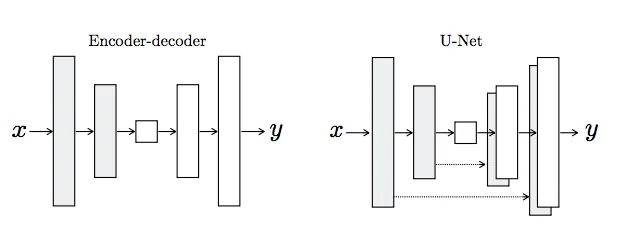
\includegraphics[width=0.5\textwidth]{model/unet-gen}
    \caption{U-Net architecture}
    \label{fig:unet}
\end{figure}
\subsection{PatchGAN Discriminator}
\label{subsec:patchgan-discriminator}
The discriminator is a convolutional neural network that classifies the real and fake
images. The discriminator architecture is such that each convolutional block in the
discriminator consists of a convolution layer, a batch normalization layer, and a Leaky
ReLU activation layer. The PatchGAN discriminator architecture is such that it only penalizes
the structure at the scale of patches. This discriminator tries to classify if each N x N
patch in an image is real or fake.
\begin{figure}[H]
    \centering
    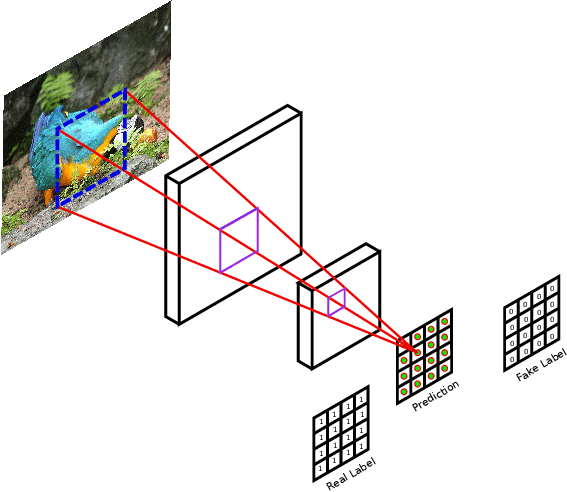
\includegraphics[width=0.5\textwidth]{model/patch-gan}
    \caption{PatchGAN discriminator.\\ Each value of the output matrix represents the probability of whether the corresponding image patch is real or it is artificially generated.}
    \label{fig:patchgan}
\end{figure}
\subsection{Training process}
\label{subsec:training-process}
The training process of the model is the following:
\begin{enumerate}
    \item The generator G takes the input image X and generates the output image Y'.
    \item The discriminator D takes the input image X and the generated image Y' and
    classifies them as real or fake.
    \item The generator loss is calculated as the sum of adversarial loss and L1 loss.
    \item The discriminator loss is the sum of the losses for the real and fake images.
    \item The generator and discriminator parameters are updated using the gradients
    obtained in the previous step.
\end{enumerate}
\begin{figure}[H]
    \centering
    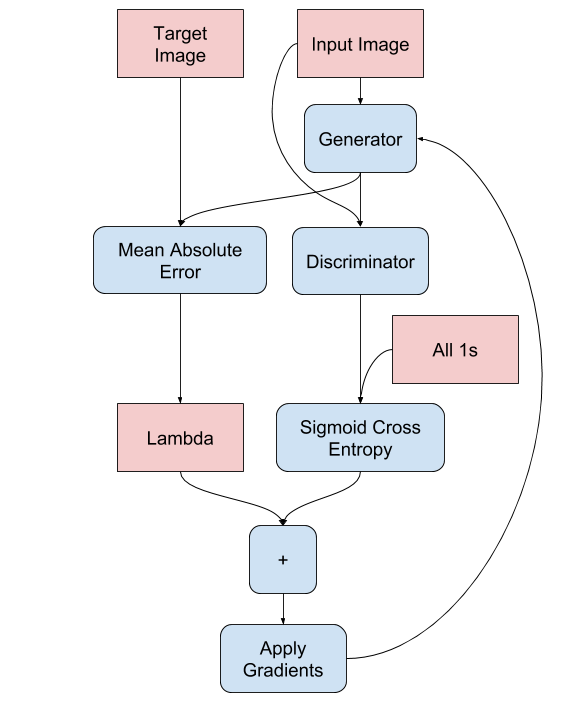
\includegraphics[width=0.50\textwidth]{model/gen-training}
    \caption{Generator training process}
    \label{fig:gen-training}
    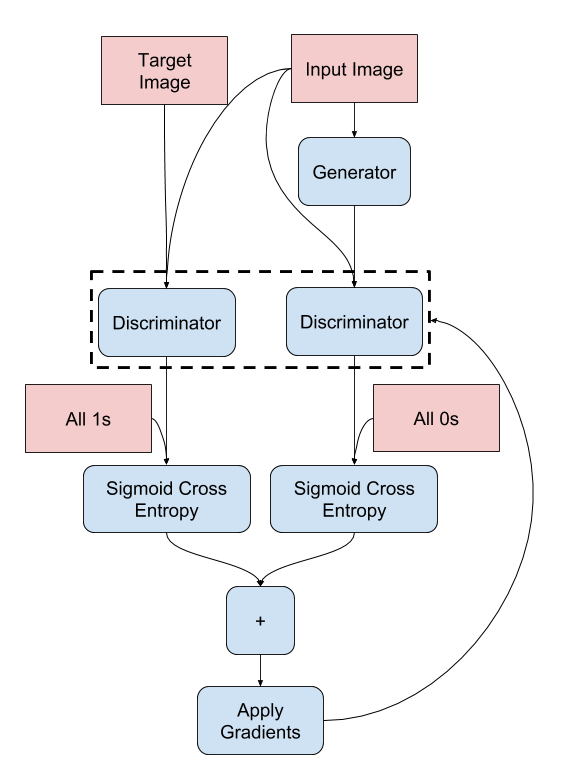
\includegraphics[width=0.50\textwidth]{model/dis-training}
    \caption{Discriminator training process}
    \label{fig:dis-training}
\end{figure}
\subsection{User Interface}
\label{subsec:user-interface}
The user interface was developed using the Python library Tkinter.
It consists of a window with a menu bar and a canvas where the user can draw.
The menu bar consists of the following:
\begin{itemize}
    \item \textbf{Colors}
    \begin{itemize}
        \item \textbf{Brush Color}: Set the Brush color.
        \item \textbf{background Color}: Set the background color.
    \end{itemize}
    \item \textbf{Options}
    \begin{itemize}
        \item \textbf{Clear canvas}: Undo the last action.
        \item \textbf{Generate Image}: Redo the last action.
        \item \textbf{Load CAD}: Load a CAD file as input.
        \item \textbf{Load PNG/JPG}: Load a .PNG file as input.
        \item \textbf{Exit}: Exit the application.
    \end{itemize}
\end{itemize}
\begin{figure}[H]
    \centering
    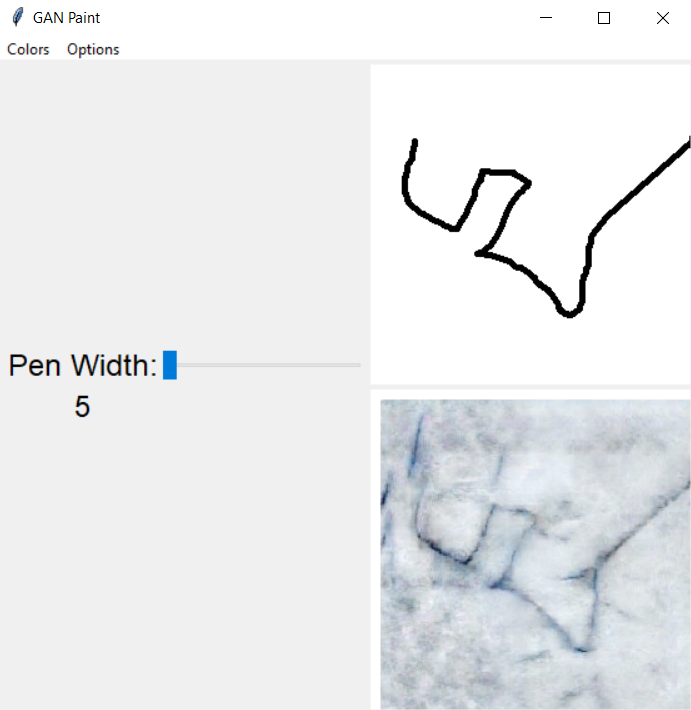
\includegraphics[width=0.50\textwidth]{ui/ui}
    \caption{User interface}
    \label{fig:ui}
\end{figure}
Once the input is submitted, the application will show the output in the lower canvas.
And save it in the \textit{output} folder.
\section{Progettazione}
\label{sec:progettazione}




\section{Design Pattern utilizzati}

\section{Codifica}
